\chapter{Разработка прототипа инструмента обнаружения клонов}

В данном разделе приводится подробное описание реализации прототипа инструмента обнаружения клонов. А именно, рассматривается общая структура прототипа, реализация <<мутатора>> и нейронных сетей.

\section{Общая структура прототипа}

Общая структура прототипа показана на рис.~\ref{fig:clones_prot}. Разрабатываемый прототип инструмента обнаружения клонов состоит и двух модулей:
\begin{itemize}
\setlength\itemsep{0mm}
\item Модуль построения AST - выполняет все операции, связанные с предобработкой и преобразованием;
\item Модуль поиска клонов с помощью НС - выполняет поиск клонов.
\end{itemize}

\begin{figure}[htbp]
\centering
\includegraphics[width=0.6\textwidth]{clonesstruct.png}
\caption{Общая структура прототипа}
\label{fig:clones_prot}
\end{figure}

Как было описано ранее, языком реализации модуля построения AST и представления его в виде токенов был выбран Java. Реализация модуля поиска клонов была выполнена с помощью популярной программной платформы от Google -  Tensorflow. Языком реализации является Python.

\section{Реализация модуля построения AST}

Структура разрабатываемого модуля показана на рис.~\ref{fig:astmod}. Данный модуль состоит из нескольких основных программных пакетов:

\begin{itemize}
\setlength\itemsep{0mm}
\item \texttt{trees} - реализует построение AST из заданного исходного кода;
\item \texttt{preproc} - обеспечивает преобразование AST в последовательность токенов. Также отвечает за векторное представление токенов;
\item \texttt{postgresql} - реализует общение с базой данных PostgreSQL в случае использования BigCloneBench.
\end{itemize}


\begin{figure}[htbp]
\centering
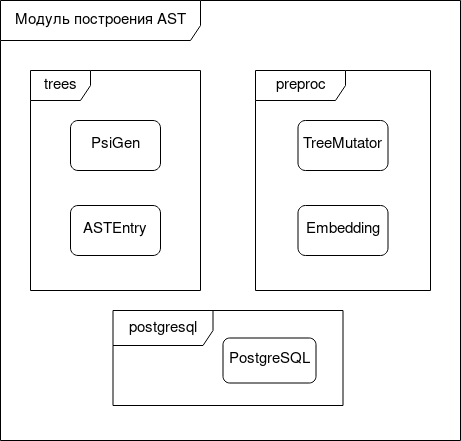
\includegraphics[width=0.7\textwidth]{astmod.png}
\caption{Структура модуля построения AST}
\label{fig:astmod}
\end{figure}

\subsection{Состав пакета trees}

Данный пакет содержит классы, обеспечивающие преобразование исходного кода в абстрактное дерево. На самом деле, данный пакет создает PSI (Program Structure Interface), что можно рассматривать как расширение AST. В данный пакет входят два класса:

\begin{itemize}
\setlength\itemsep{0mm}
\item \texttt{PsiGen} - класс, отвечающий за анализ исходного кода программы и создания из него PSI. Помимо создания PSI, рассматриваемый класс преобразует PSI в последовательность токенов.
\item \texttt{ASTEntry} - представляет из себя реализацию токенов, которые используются в дальнейшем. Также данный класс содержит в себе различные методы взаимодействия с токенами.
\end{itemize}

\nomenclature{PSI}{Program Structure Interface}

Далее будет приведено описание класса ASTEntry.

\subsubsection{ASTEntry}

Как было описано выше, данный класс представляет из себя реализацию токена, входящего в PSI. Данный класс включает в себя следующие элементы класса:

\begin{itemize}
\setlength\itemsep{0mm}
\item \texttt{nodeName} - элемент класса, содержащий в себе имя узла;
\item \texttt{sourceStart} - элемент класса, определяющий строку, где начинается данный токен;
\item \texttt{sourceEnd} - элемент класса, определяющий строку, где заканчивается данный токен;
\item \texttt{parent} - элемент класса, указывающий на родителя токена;
\item \texttt{children} - список всех дочерних токенов для рассматриваемого;
\item \texttt{filePath} - содержит в себе путь файла из которого был извлечен данный токен;
\end{itemize}

и следующие методы:

\begin{itemize}
\setlength\itemsep{0mm}
\item \texttt{removeSpaces} - метод, производящий удаление неинтересующих нас токенов из списка дочерних;
\item \texttt{getAllTokensList} - метод, который обходит список всех дочерних токенов и возвращает только их имена в виде списка;
\item \texttt{filePath} - содержит в себе путь файла из которого был извлечен данный токен;
\item \texttt{mutate} - метод, производящий мутации различного типа;
\end{itemize}

\subsection{Состав пакета preproc}

В пакет preproc	входят классы отвечающие за создание векторных представлений токенов и мутации этих токенов:

\begin{itemize}
\setlength\itemsep{0mm}
\item \texttt{TreeMutator} - данный класс организует работу с исходным кодом. А именно - вызывает создание PSI, выполняет преобразование PSI в последовательность токенов, производит ее фильтрацию и, при необходимости - мутацию;
\item \texttt{Embedding} - реализует создание векторных представлений токенов и записывает полученные результаты в файлы. Таким образом, данный класс организует создание выборки данных для последующего обучения сетей.
\end{itemize}

Далее рассматривается класс Embedding, т.к. он представляет наибольший интерес.

\subsubsection{Embedding}

Рассматриваемый класс содержит в себе реализацию word2vec с помощью которой производится создание векторных представлений. В данный класс входят следующие методы:

\begin{itemize}
\setlength\itemsep{0mm}
\item \texttt{train} - метод, который осуществляет обучение модели word2vec на заранее выбранном проекте. В нашем случае, в качестве данного проекта был выбран openjdk. В данном методе, также, производится сериализация обученной модели с целью ее повторного использования. 
\item \texttt{createEmbedding} - метод, отвечающий за создание векторного представления заданных токенов и сохранение их в файл.
\end{itemize}

\section{Реализация модуля обнаружения программных клонов}

Структура модуля поиска клонов показана на рис.~\ref{fig:clonedet}. Данный модуля был написан с использованием платформы Tensorflow. Он состоит из нескольких файлов, в которых описаны различные классы и методы:

\begin{itemize}
\setlength\itemsep{0mm}
\item \texttt{clonesRecognition} - основной файл, в котором организуется работа с инструментом. Вызываются различные методы инициализации, обучения, вычисления и т.д.;
\item \texttt{model} - файл, в котором описываются модели нейронных сетей, методы их обучения и использования;
\item \texttt{helpers} - вспомогательный файл, в котором описываются различные методы преобразования информации, сохранения, чтения и т.п.;
\end{itemize}

\begin{figure}[htbp]
\centering
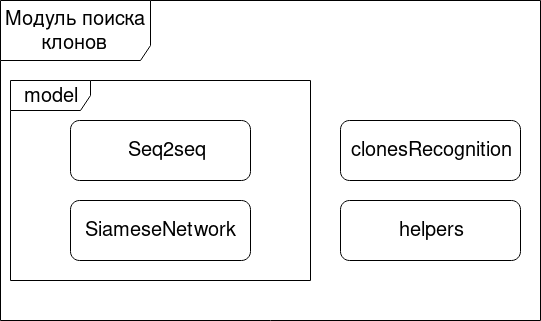
\includegraphics[width=\textwidth]{clonedet.png}
\caption{Структура модуля поиска клонов}
\label{fig:clonedet}
\end{figure}

\subsection{Состав файла model}

Как уже было описано, в данном файле содержатся два класса, описывающих разные НС:

\begin{itemize}
\setlength\itemsep{0mm}
\item \texttt{Seq2seq} - класс, реализующий seq2seq алгоритм;
\item \texttt{SiameseNetwork} - класс, реализующий Сиамскую архитектуру НС.
\end{itemize}

\subsubsection{Seq2seq}

В рассматриваемом классе присутствуют следующие элементы:

\begin{itemize}
\setlength\itemsep{0mm}
\item \texttt{scope} - содержит в себе название предела, в котором будут существовать все переменные (необходим для корректной сериализации и десереализации обученной модели);
\item \texttt{sess} - сессия внутри которой будут проходить обучение и вычисления;
\item \texttt{encoder\_cell} - ячейка кодировщика (отвечает за попытки привести информацию к вектору фиксированного размера);
\item \texttt{decoder\_cell} - ячейка декодировщика;
\item \texttt{vocab\_size} - размер словаря (в нашем случае - длинна векторного представления токена);
\item \texttt{input\_embedding\_size} - размер входной последовательности.
\end{itemize}

Помимо указанных элементов, в данном классе присутствуют методы обучения (train) и вычисления (get\_encoder\_status).

\subsubsection{SiameseNetwork}

Так как в данном классе присутствуют элементы схожие с элементами предыдущего класса, в этом подразделе они рассмотрены не будут. Рассмотрим отличающиеся элементы:

\begin{itemize}
\setlength\itemsep{0mm}
\item \texttt{input\_x1} - переменная первой последовательности для сравнения;
\item \texttt{input\_x2} - переменная второй последовательности для сравнения;
\item \texttt{input\_y} - переменная указывающая на сходство/различие первых двух (0 - схожи, 1 - различны);
\item \texttt{sequence\_length} - переменная, указывающая длину последовательности (результат работы seq2seq)
\item \texttt{layers} - количество слоев для обучения
\end{itemize}

\subsection{Состав файла helpers}

В файле helpers содержатся только вспомогательные методы. Среди них:

\begin{itemize}
\setlength\itemsep{0mm}
\item \texttt{batch} - создает серии значений из заданной последовательности;
\item \texttt{siam\_batches} - представляет заданные параметры для обучения Сиамской сети в виде тройки значений \(\{x_1, x_2, y\}\);
\item \texttt{random\_sequences} - производит генерацию случайных последовательностей для обучения seq2seq модели;
\item \texttt{save\_model} - производит сохранение модели в указанный файл;
\item \texttt{load\_model} - производит загрузку модели из указанного файла.
\end{itemize}

\subsection{Состав файла clonesRecognition}

Как упоминалось ранее, данный файл является входной точкой рассматриваемой утилиты. В нем содержатся следующие методы:

\begin{itemize}
\setlength\itemsep{0mm}
\item \texttt{main} - входная точка утилиты. В ней производится инициализация основных значений, выбор типа работы (обучение, расчет или полный);
\item \texttt{seq2seq\_train} - обучение seq2seq модели;
\item \texttt{siam\_train} - обучение Сиамской НС;
\item \texttt{eval} - производит полный расчет;
\end{itemize}

\section{Итоги раздела}

В данном разделе была рассмотрена реализация прототипа инструмента обнаружения клонов, основанного на предложенном интеллектуальном методе анализа. Приведена общая структура прототипа и описаны его основные составляющие: инструмент предобработки и инструмент обнаружения клонов.
